\chapter{Лабораторная работа №5 (4/2)\\
Измерение ослабления ступенчатого аттенюатора}

\section{Цель работы}

Изучить теоретические основы измерений коэффициентов отражения и ослаблений на СВЧ:
\begin{itemize}
    \item определения измеряемых величин;
    \item единицы величин;
    \item принцип и метод измерений величин «по определению»;
    \item операции, выполняемые при измерении;
    \item физические явления, выражающие погрешности измерений.
\end{itemize}

% \section{Теоретические сведения}

\section{Пратическая часть}

В соответствии с методическими указаниями проведём измерения и занесём полученные данные в таблицу~\ref{tab:attenuations}.

\begin{table}[H]
    \centering
    \caption{Ослабления}%
    \label{tab:attenuations}
    \resizebox{\textwidth}{!}{%
        \begin{tabular}{@{}lcccccccccc@{}}
            \toprule
            Частота \\ Установка атт. & 4.8--4.9 & 4.9--5.0 & 5.0--5.1 & 5.1--5.2 & 5.2--5.3 & 5.3--5.4 & 5.4--5.5 & 5.5--5.6 & Ср. знач. & $\Delta A = A_\text{изм} - A_\text{дейст}$ \\ \midrule
            1                         & -1.2     & -0.8     & -0.8     & -0.7     & -0.8     & -1.0     & -1.0     & -0.9     & -0.9      & 0.10                                       \\
            2                         & -1.7     & -1.9     & -1.9     & -1.7     & -1.7     & -1.9     & -2.0     & -2.0     & -1.9      & 0.15                                       \\
            4                         & -3.6     & -3.6     & -3.6     & -3.2     & -3.6     & -3.6     & -3.6     & -3.6     & -3.6      & 0.45                                       \\
            4                         & -3.6     & -3.6     & -3.6     & -3.2     & -3.6     & -3.6     & -3.6     & -3.6     & -3.6      & 0.45                                       \\
            10                        & -10.3    & -9.4     & -9.4     & -9.0     & -9.2     & -9.2     & -9.8     & -10.8    & -9.6      & 0.36                                       \\
            20                        & -19.2    & -18.8    & -18.9    & -18.4    & -18.6    & -18.8    & -18.8    & -19.0    & -18.8     & 1.19                                       \\
            1+2                       & -2.6     & -2.6     & -2.7     & -2.3     & -2.6     & -2.7     & -2.7     & -2.8     & -2.6      & 0.38                                       \\
            1+4                       & -4.4     & -4.6     & -4.4     & -3.8     & -4.6     & -5.3     & -4.1     & -4.4     & -4.5      & 0.55                                       \\
            2+4                       & -5.5     & -5.6     & -5.7     & -4.6     & -4.8     & -5.0     & -6.2     & -6.8     & -5.5      & 0.48                                       \\
            2+4+4                     & -9.8     & -9.4     & -9.6     & -9.0     & -9.4     & -9.4     & -10.2    & -11.0    & -9.7      & 0.28                                       \\
            2+10                      & -12.3    & -11.4    & -11.6    & -11.4    & -11.6    & -11.8    & -11.8    & -12.1    & -11.8     & 0.25                                       \\
            4+10                      & -13.6    & -13.2    & -13.6    & -13.0    & -13.2    & -13.6    & -13.6    & -13.6    & -13.4     & 0.58                                       \\
            4+4+10                    & -17.5    & -17.3    & -17.3    & -17.1    & -17.4    & -17.6    & -17.6    & -17.5    & -17.4     & 0.59                                       \\
            2+4+4+10                  & -19.4    & -19.0    & -19.0    & -18.6    & -19.0    & -19.2    & -19.2    & -19.2    & -19.1     & 0.93                                       \\
            2+4+20                    & -24.4    & -23.8    & -23.8    & -23.4    & -23.8    & -24.0    & -24.0    & -24.4    & -24.0     & 2.05                                       \\
            10+20                     & -26.5    & -26.4    & -26.5    & -26.3    & -26.6    & -27.0    & -27.2    & -27.3    & -26.7     & 3.28                                       \\
            2+4+4+10+20               & -28.6    & -28.6    & -29.2    & -28.6    & -29.4    & -30.3    & -30.6    & -31.2    & -29.6     & 10.44                                      \\ \bottomrule
        \end{tabular}%
    }
\end{table}

На основе полученных данных построим зависимость ошибки от ослабления (Рис.~\ref{fig:attenuation-error}).

\begin{figure}[H]
    \centering
    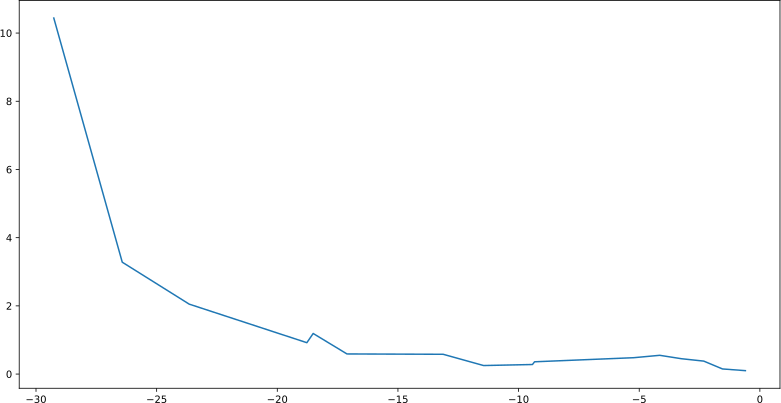
\includegraphics[width=\textwidth]{attenuation-error}
    \caption{Зависимость ошибки от ослабления}%
    \label{fig:attenuation-error}
\end{figure}

\section{Ответы на вопросы}

Ответы на вопросы даны в лабораторной работе №2 (4/1).
